
\section{System Design} : Systems design is the process or art of defining the architecture, components, modules, interfaces, and data for a system to satisfy specified requirements. One could see it as the application of systems theory to product development. There is some overlap with the disciplines of systems analysis, systems architecture and systems engineering.
\begin{itemize}
\item  External design: External design consists of conceiving, planning out and specifying the externally observable characteristics of the software product. These characteristics include user displays or user interface forms and the report formats, external data sources and the functional characteristics, performance requirements etc. External design begins during the analysis phase
and continues into the design phase.
\item  Logical design: The logical design of a system pertains to an abstract representation of the data flows, inputs and outputs of the system. This is often conducted via modeling, which involves a simplistic (and sometimes graphical) representation of an actual system. In the context of systems design, modelling can undertake the following forms, including:
\begin{itemize}
\item Data flow diagrams
\item Entity Relationship Diagrams
\end{itemize}
\item  Physical design: The physical design relates to the actual input and output processes of the system. This is laid down in terms of how data is input into a system, how it is verified/authenticated, how it is processed, and how it is displayed as output.
\end{itemize}

\section{Design Notations}
\newpage
\noindent Data Flow diagrams:
\begin{figure}[h]
\centering 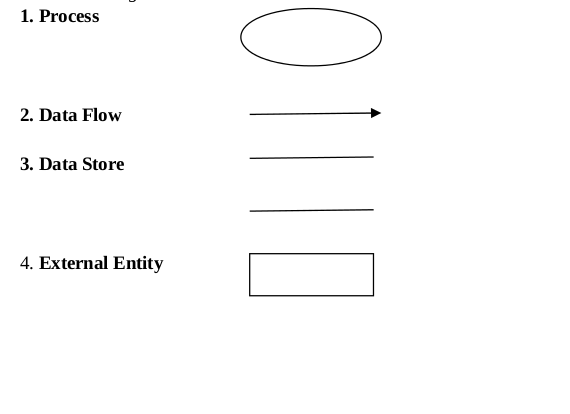
\includegraphics[scale=0.6]{images/sss1.png}
\end{figure}

\noindent Flow Charts:
\begin{figure}[h]
\centering 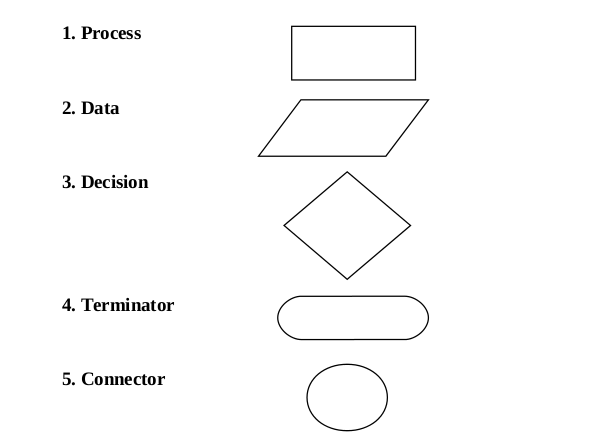
\includegraphics[scale=0.5]{images/sss2.png}
\end{figure}
\newpage
Entity Relationship Diagrams:
\begin{figure}[h]
\centering 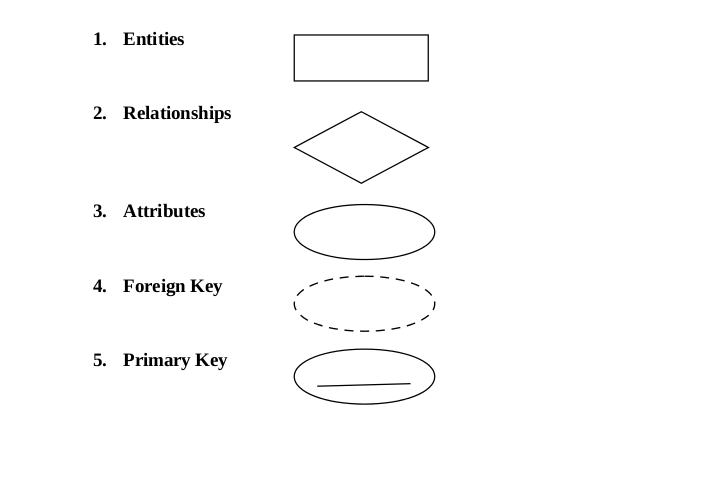
\includegraphics[scale=0.5]{images/sss3.png}
\end{figure}\\
 \section{Detailed Design}
We basically describe the functionality of the system internally. The internal design describes how data is
flowing from database to the user and how they both are internally connected. For this reason we can show
the design of the system in detailed manner by many ways:\\
{\bf Flowchart } A flowchart is a type of diagram that represents an algorithm or process, showing the steps as boxes of various kinds, and their order by connecting them with arrows. This diagrammatic representation can give a step-by-step solution to a given problem. Process operations are represented in these boxes, and arrows connecting them represent flow of control. Data flows are not typically represented in a flowchart, in contrast with data flow diagrams; rather, they are implied by the sequencing of operations. Flowcharts are used in analyzing, designing, documenting or managing a process or program in various fields

\newpage
\begin{figure}[h]
\centering 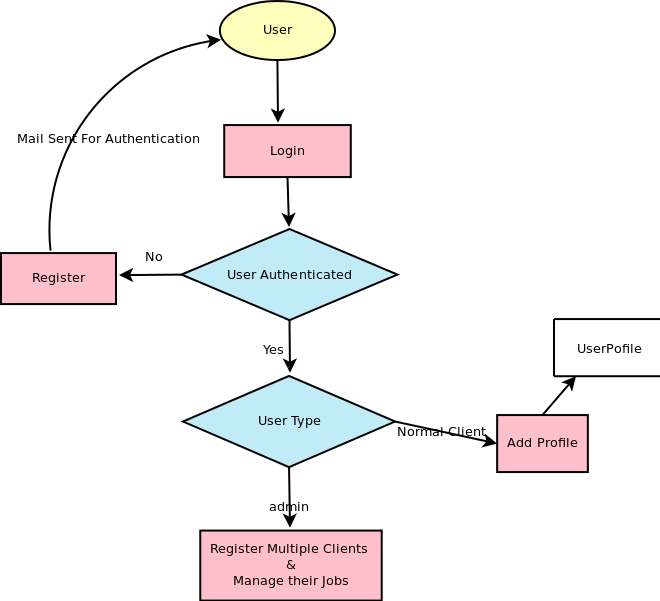
\includegraphics[scale=0.8]{images/register.png}
\caption{Flow Chart for Registeration}
\end{figure} 
\newpage
\begin{figure}[h]
\vskip 3cm
\centering 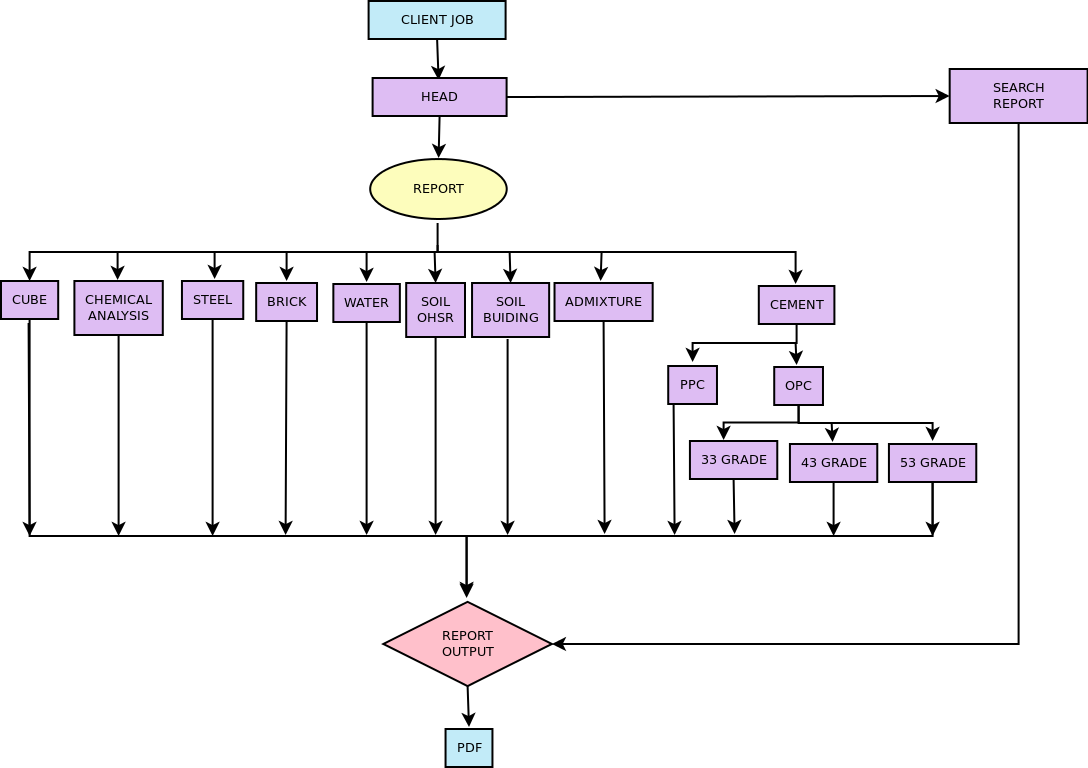
\includegraphics[scale=0.45]{images/report.png}
\caption{Flow Chart for Reports}
\end{figure} 
\newpage
\begin{figure}[h]

\centering 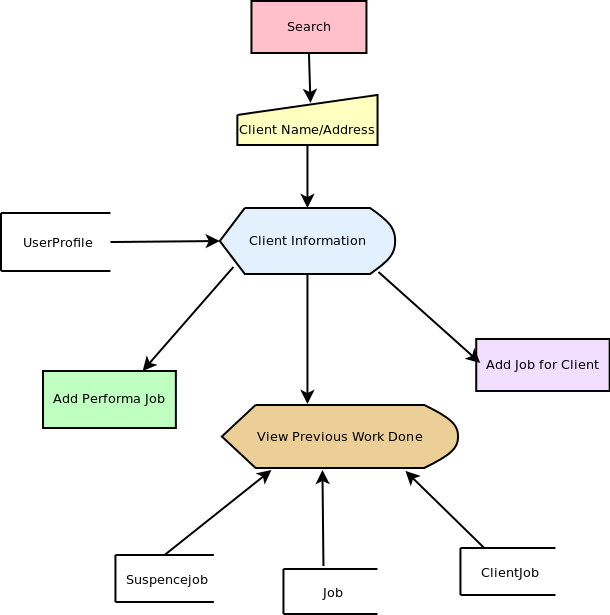
\includegraphics[scale=0.7]{images/search.png}
\caption{Flow Chart for Searching a Client}
\end{figure}

\newpage
\begin{figure}[h]
\centering 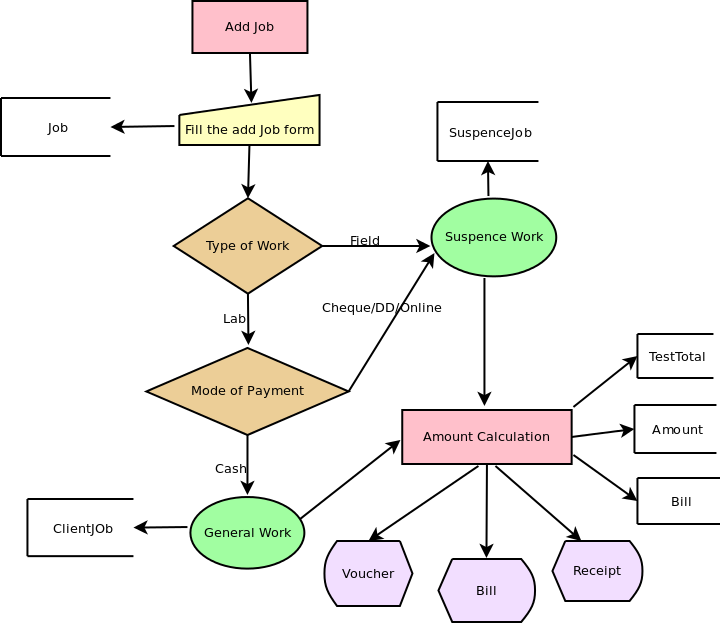
\includegraphics[scale=0.7]{images/addjob.png}
\caption{Flow Chart for adding a Job}
\end{figure}

\newpage
\begin{figure}[h]
\centering 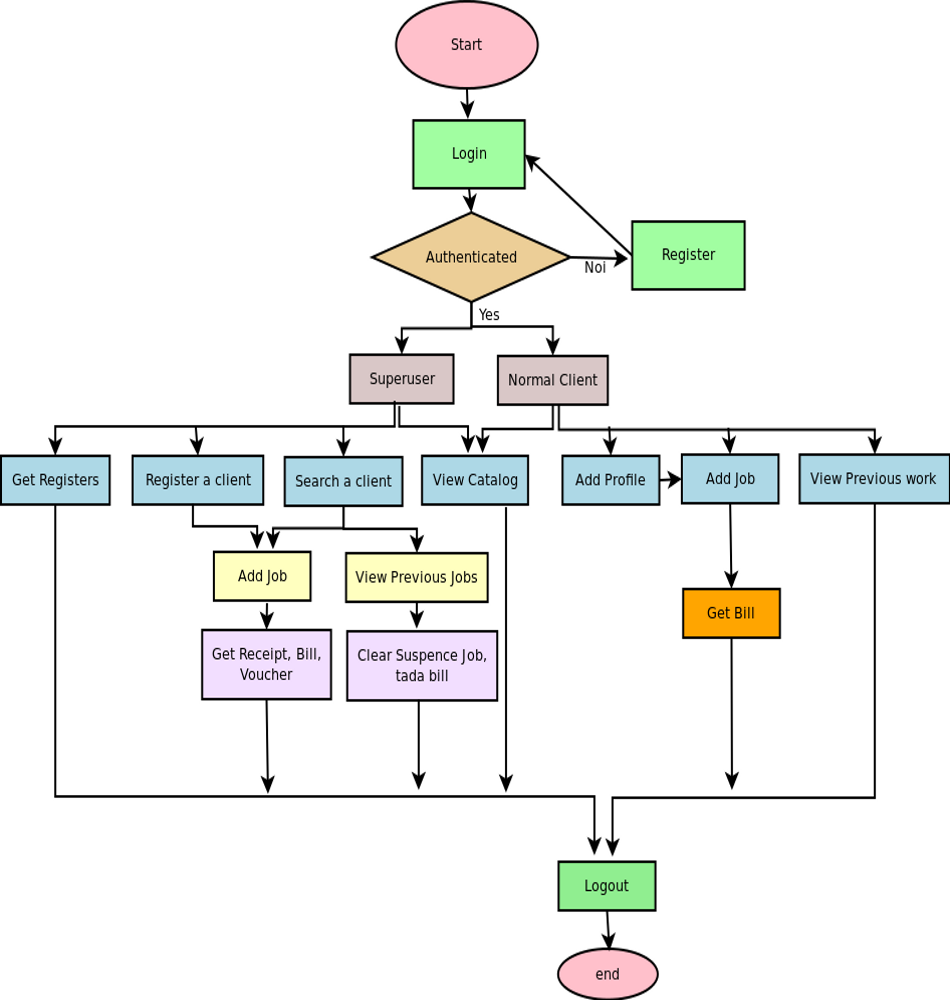
\includegraphics[scale=0.5]{images/automation.png}
\caption{Flow Chart for software}
\end{figure}
\newpage

\begin{figure}[h]
\centering 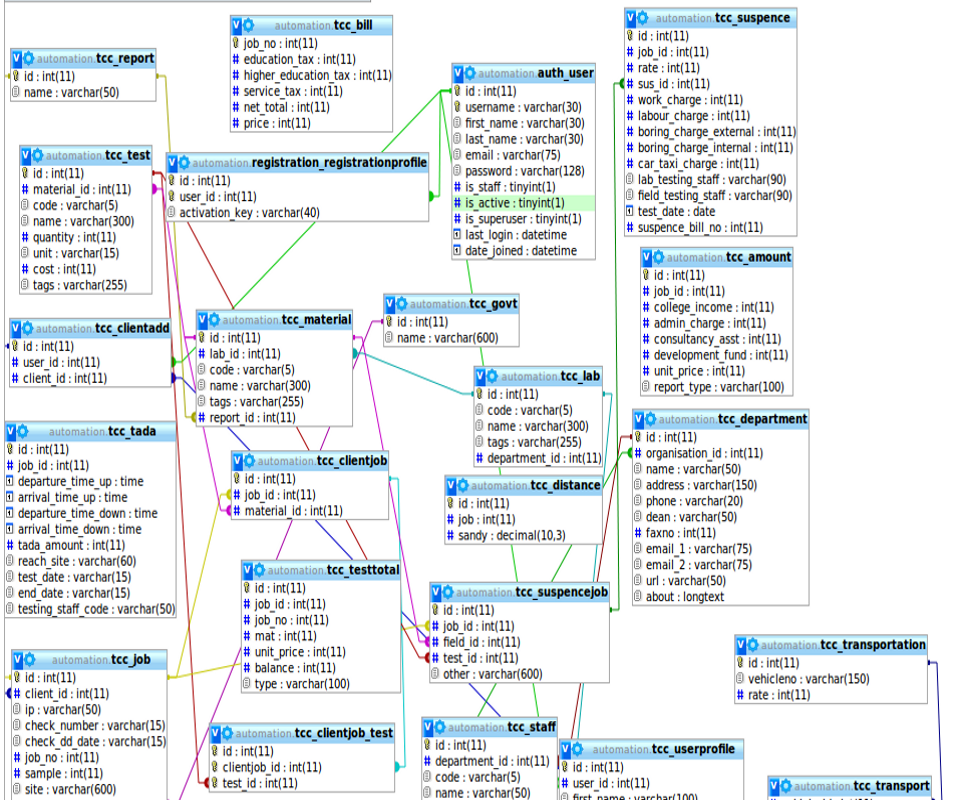
\includegraphics[scale=0.5]{images/db1.png}
\centering 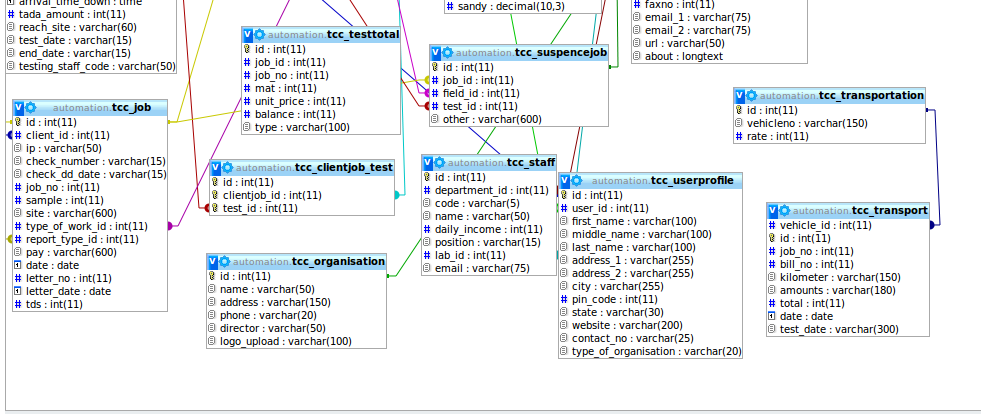
\includegraphics[scale=0.5]{images/db2.png}
\caption{Database Design}
\end{figure}
\newpage

